\documentclass[english,notitlepage]{revtex4-1}  % defines the basic parameters of the document
%For preview: skriv i terminal: latexmk -pdf -pvc filnavn



% if you want a single-column, remove reprint

% allows special characters (including æøå)
\usepackage[utf8]{inputenc}
%\usepackage[english]{babel}

%% note that you may need to download some of these packages manually, it depends on your setup.
%% I recommend downloading TeXMaker, because it includes a large library of the most common packages.

\usepackage{physics,amssymb}  % mathematical symbols (physics imports amsmath)
\include{amsmath}
\usepackage{graphicx}         % include graphics such as plots
\usepackage{xcolor}           % set colors
\usepackage{hyperref}         % automagic cross-referencing (this is GODLIKE)
\usepackage{listings}         % display code
\usepackage{subfigure}        % imports a lot of cool and useful figure commands
\usepackage{float}
%\usepackage[section]{placeins}
\usepackage{algorithm}
\usepackage[noend]{algpseudocode}
\usepackage{subfigure}
\usepackage{tikz}
\usetikzlibrary{quantikz}
% defines the color of hyperref objects
% Blending two colors:  blue!80!black  =  80% blue and 20% black
\hypersetup{ % this is just my personal choice, feel free to change things
    colorlinks,
    linkcolor={red!50!black},
    citecolor={blue!50!black},
    urlcolor={blue!80!black}}

%% Defines the style of the programming listing
%% This is actually my personal template, go ahead and change stuff if you want



%% USEFUL LINKS:
%%
%%   UiO LaTeX guides:        https://www.mn.uio.no/ifi/tjenester/it/hjelp/latex/
%%   mathematics:             https://en.wikibooks.org/wiki/LaTeX/Mathematics

%%   PHYSICS !                https://mirror.hmc.edu/ctan/macros/latex/contrib/physics/physics.pdf

%%   the basics of Tikz:       https://en.wikibooks.org/wiki/LaTeX/PGF/Tikz
%%   all the colors!:          https://en.wikibooks.org/wiki/LaTeX/Colors
%%   how to draw tables:       https://en.wikibooks.org/wiki/LaTeX/Tables
%%   code listing styles:      https://en.wikibooks.org/wiki/LaTeX/Source_Code_Listings
%%   \includegraphics          https://en.wikibooks.org/wiki/LaTeX/Importing_Graphics
%%   learn more about figures  https://en.wikibooks.org/wiki/LaTeX/Floats,_Figures_and_Captions
%%   automagic bibliography:   https://en.wikibooks.org/wiki/LaTeX/Bibliography_Management  (this one is kinda difficult the first time)
%%   REVTeX Guide:             http://www.physics.csbsju.edu/370/papers/Journal_Style_Manuals/auguide4-1.pdf
%%
%%   (this document is of class "revtex4-1", the REVTeX Guide explains how the class works)


%% CREATING THE .pdf FILE USING LINUX IN THE TERMINAL
%%
%% [terminal]$ pdflatex template.tex
%%
%% Run the command twice, always.
%% If you want to use \footnote, you need to run these commands (IN THIS SPECIFIC ORDER)
%%
%% [terminal]$ pdflatex template.tex
%% [terminal]$ bibtex template
%% [terminal]$ pdflatex template.tex
%% [terminal]$ pdflatex template.tex
%%
%% Don't ask me why, I don't know.

\begin{document}

\title{FYS3150 oppgavesett 1}

\author{Jon Aleksander Prøitz and Marius Torsvoll}


\begin{abstract}
\noindent Relevant code can be found at:
\url{https://github.com/Jonaproitz/Project_1}
\end{abstract}

\noaffiliation

\maketitle
%\date{Received - / Accepted -}


\section*{Problem 1.}
    \label{sec:oppgave1}
    Given
    \begin{equation}
            u(x) 
        =   1-(1-e^{-10})x - e^{-10x}
        \label{u}
    \end{equation}
    Inserting $x = 0$ 
    \begin{equation*}
            u(0)
        =   1 - (1 - e^{-10}) \cdot 0 - e^{-10 \cdot 0}
        =   1 - 0 - 1
        =   0
    \end{equation*}
    and $x = 1$
    \begin{equation*}
            u(1)
        =   1 - (1 - e^{-10}) \cdot 1 - e^{-10 \cdot 1}
        =   1 - 1 + e^{-10} - e^{-10}
        =   0
    \end{equation*}
    furthermore the one-dimensional possion equation can be written
    \begin{equation*}
            -\frac{d^2 u}{d x^2} 
        =   -\frac{d^2}{d x^2}\left(1-(1-e^{-10})x - e^{-10x}\right)
        =   -\frac{d}{d x}\left((1-e^{-10}) + 10e^{-10x} \right) 
        =   100e^{-10x}
        =   f(x)
    \end{equation*}
    Hence equation \ref{u} is an exact solution to our problem.
    \hfill$\blacksquare$


\section*{Problem 2.}
    \label{sec:oppgave2}
    \begin{figure}[!ht]
        \centering
        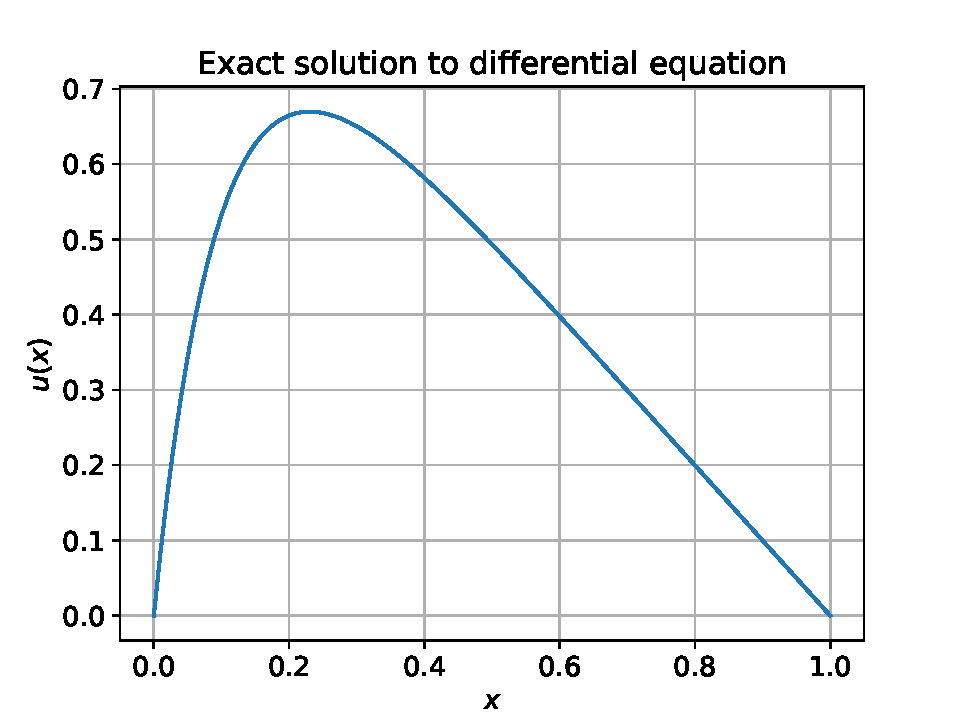
\includegraphics[scale=0.7]{exact_solution.pdf}
        \caption{Plot of equation \ref{u} in the given area $x \in [0, 1]$.}
        \label{exact_plot}
    \end{figure}


\section*{Problem 3.}
    The one-dimensional poisson equation can be written
    \begin{equation*}
            -\frac{d ^2 u}{dx^2} 
        =   \frac{u(x-h)+2u(x)- u(x+h)}{h^2} + O(h^2)
        =   f(x)
    \end{equation*}
    Discretizing $x$ with $m$ values and a given distance $h$ between each distinct value then gives
    \begin{align*}
            x 
        \rightarrow 
            x_0, x_1, x_2, ..., x_{m - 1}\\
            u(x) 
        \rightarrow 
            u_0, u_1, u_2, ..., u_{m - 1}\\
            f(x) 
        \rightarrow 
            f_0, f_1 , f_2, ..., f_{m - 1}
    \end{align*}
    with $u_i = v_i$, such that
    \begin{equation*}
            -\frac{d^2 v_i}{dx^2} 
        =   -v_{i-1} + 2v_i - v_{i+1} 
        =   f_ih^2
    \end{equation*}


\section*{Problem 4.}
    \label{sec:oppgave4}
    The set of equations from problem 3 can be written as 
    \begin{align*}
            -v_0 + 2v_1 - v_2 
        &=  h^2 f_1\\
            -v_1 + 2v_2 -v_3 
        &=  h^2 f_2\\
            -v_2 + 2v_3- v_4 
        &=  h^2 f_3\\
        \vdots&\\
            -v_{m-3} + 2 v_{m-2} - v_{m - 1}
        &=  h^2 f_{m-2}
    \end{align*}
    Wich for 
    \begin{align*}
            g_1
        =&  h^2 f_1 + v_0\\
            g_2
        =&  h^2 f_2\\
            g_3
        =&  h^2 f_3\\
        &\vdots\\
            g_{m - 3}
        =&  h^2 f_{m-3}\\
            g_{m-1}
        =&  h^2 f_{m-2} + v_{m - 1}
    \end{align*}
    can be written as the matrix equation
    \begin{equation*}
            \begin{pmatrix}
                2 & -1 & 0 &0 & 0 & \dots
                \\
                -1 & 2 & -1 & 0 & 0 & \dots
                \\
                0 & -1 & 2 & -1 & 0 & \dots
                \\
                \vdots & \vdots & \ddots & \ddots & \ddots
                \\
                0 & 0 & 0 & -1 & 2 & -1
                \\ 
                0 & 0 & 0 & 0 & -1 & 2 
            \end{pmatrix}
            \begin{pmatrix}
                v_1 \\ v_2 \\ v_3 \\ \vdots \\ v_{m - 3} \\ v_{m - 2} 
            \end{pmatrix} 
        =   \begin{pmatrix}
                g_1 \\ g_2 \\ g_3 \\ \vdots \\ g_{m - 3} \\ g_{m - 2}
            \end{pmatrix}
    \end{equation*}
    on the form $A\vec{v} = \vec{g}$.


\section*{Problem 5}
    \subsection*{a}
        \label{sec:oppgave5a}
        When finding the matrix, $A$, in problem 4 it is assumed that $v_0$ and $v_{m - 1}$ are known.
        Hence theese values are not calculated and
        \begin{equation*}
                n
            =   m - 2
        \end{equation*}
    
    \subsection*{b}
        \label{sec:5b}
        As discussed above the the vector $\vec{v}$ is equal to $\vec{v}^*$ excluding the first and last element.
        Hence
        \begin{equation}
            \vec{v}^* = \left[v_0, \vec{v}, v_{m - 1} \right]
        \end{equation}


\section*{Problem 6}
    \subsection*{a}
        \label{sec:6a}
        A general tridiagonal matrix is given by the following: syntax: 
        \begin{equation}
            \begin{matrix}
                (R_1) & b_1 & c_1 & 0 &0 & 0 & \dots & | & g_1
                \\
                (R_2) & a_2 & b_2 & c_2 & 0 & 0 & \dots & | & g_2
                \\
                (R_3) & 0 & a_3 & b_3 & c_3 & 0 & \dots & | & g_3
                \\
                & & & &  \ddots& &  &| & \vdots
                \\
                (R_n) & 0 & 0 & 0 & 0 & a_n & b_n &|& g_n
            \end{matrix}
        \end{equation}
        Forward substitution gives us the following relation: 
        \begin{equation*}
                R_2 \rightarrow R_2 - \frac{a_2}{b_1}R_1 
            =   \begin{matrix}
                    0 & b_2 - \frac{a_2}{b_1}c_1 & 0 & 0
                \end{matrix}
        \end{equation*}
        Continuing this substitution with the variables gives us the following results for the variables:
        \begin{align*}
                \tilde{b}_1 
            =   b_1
            \hspace{3mm}\text{and}\hspace{3mm}
                \tilde{b}_i 
            =   b_i - \frac{a_i}{\tilde{b}_{i-1}}c_{i-1}, 
            \hspace{5mm}\text{For i = 2,3,4....,n}\\
                \tilde{g}_1 
            =   g_1
            \hspace{3mm}\text{and}\hspace{3mm}
                \tilde{g}_i 
            =   g_i - \frac{a_i}{\tilde{g}_{i-1}}\tilde{g}_{i-1}, 
            \hspace{5mm}\text{For i = 2,3,4....,n}
        \end{align*}
        This then gives us the matrix:
        \begin{equation*}
            \begin{matrix}
            \tilde{b} & c_1 & 0 & 0 & 0 & \dots & | & \tilde{g}_1
            \\
            0 & \tilde{b}_2 & c_2 & 0 & 0 & \dots & | & \tilde{g}_2
            \\
            0 & 0 & \tilde{b}_3 & c_3 & 0 & \dots & | & \tilde{g}_3
            \\
            & & & &  \ddots&   &| & \vdots
            \\
            0 & 0 & 0 & 0 &  & \tilde{b}_n &|& \tilde{g}_n
            \end{matrix}
        \end{equation*}
        We then see that:
        \begin{equation*}
            R_n = \frac{R_n}{\tilde{b}_n} = 
            \begin{matrix}
            0 & 0 % 0 & \dots & 1
            \end{matrix}
        \end{equation*}
        and that:
        \begin{equation*}
            \frac{\tilde{g}_n}{\tilde{b_n}} = v_n
        \end{equation*}
            Bacwards substitution then gives us the following: 
        \begin{equation*}
            v_i = \frac{\tilde{g}_i - c_i v_{i+1}}{\tilde{b}_i}, \text{For i}  = n-1, n-2, n-3,  \dots 2, 1
        \end{equation*}
    \subsection*{b}
        \label{sec:6b}
        This algorithm is thus: 
        \begin{align*}
            \tilde{b}_1 
        =   b_1\\
            \tilde{b}_i 
        =   b_i - \frac{a_i}{b_{i-1}}c_{i-1}, \text{For i} = 2,3,4\dots n\\
            \tilde{g}_1 
        =   g_1
            \tilde{g}_i 
        =   g_i - \frac{a_i}{\tilde{b}_{i-1}}\tilde{g}_{i-1}, \text{For i} = 2, 3, 4 \dots n\\
            v_n 
        =   \frac{\tilde{g}_n}{\tilde{b}_n}\\
            v_i 
        =   \frac{\tilde{g}_i-c_i v_{i+1}}{\tilde{b}_i}, \text{For i} = n-1, n-2, n-3,\dots, 1 
        \end{align*}
        
        The total amount of FLOPs will then be described as the sum of FLOPs per n. Thus the FLOPs will then be described as: $$8(n-1)(+1)$$

        
\section*{Task 7}
    \begin{figure}[!ht]
        \centering
        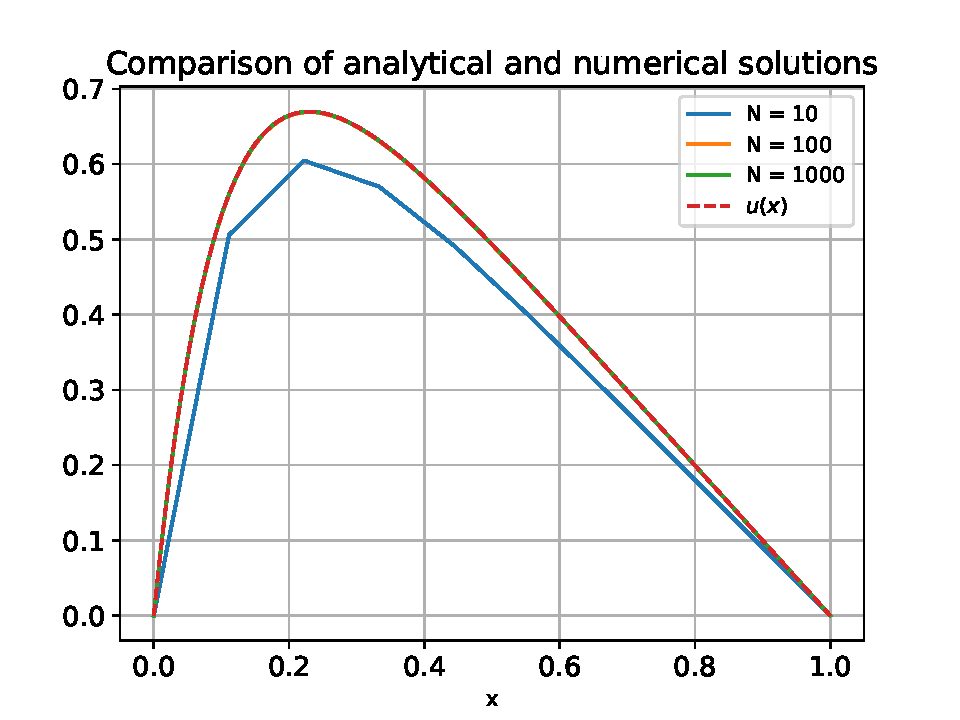
\includegraphics[scale=0.7]{comparison.pdf}
        \caption{}
        \label{comparison_plot}
    \end{figure}
        
    
\section*{Task 8}
    \begin{figure}[!ht]
        \centering
        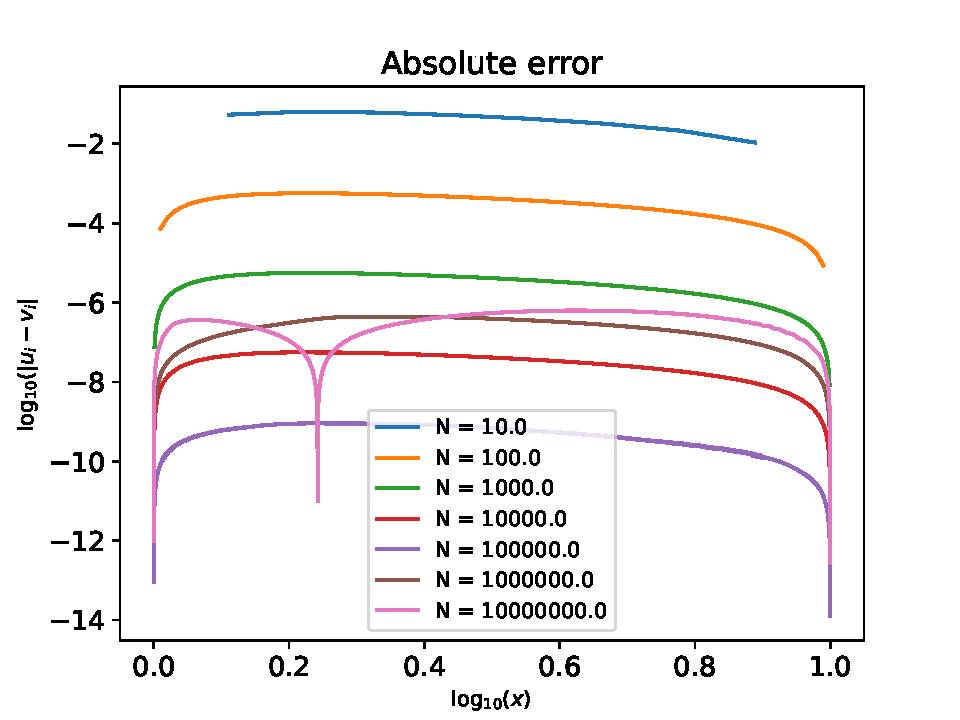
\includegraphics[scale=0.7]{abs_error.pdf}
        \caption{}
        \label{abs_error}
    \end{figure}

    \begin{figure}[!ht]
        \centering
        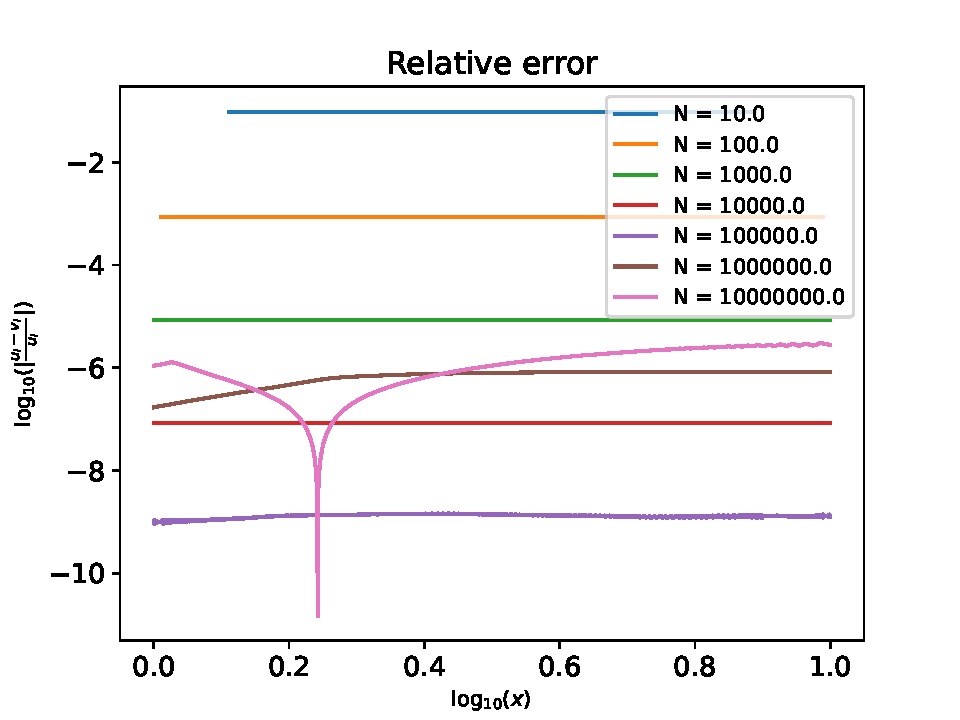
\includegraphics[scale=0.7]{rel_error.pdf}
        \caption{}
        \label{rel_error}
    \end{figure}

    \begin{figure}[!ht]
        \centering
        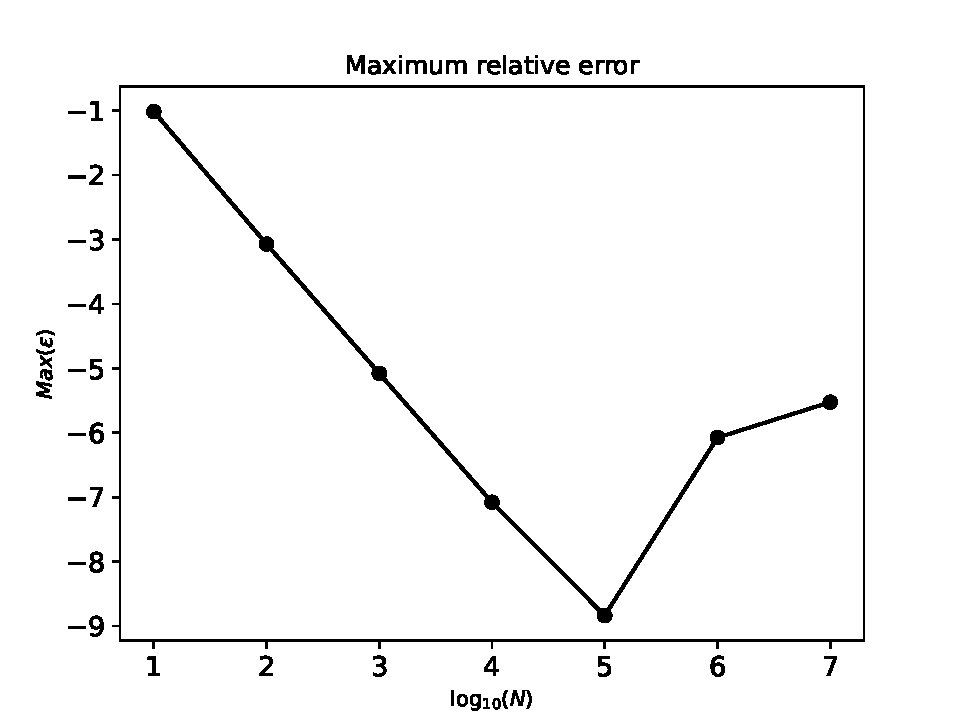
\includegraphics[scale=0.7]{max_error.pdf}
        \caption{}
        \label{max_error}
    \end{figure}


\section*{Task 9}
    \subsection*{a}
        \label{sec:9a}
        By making the special algorithm we then get the following results. 
        \begin{align*}
                \tilde{b}_1 
            =   2\\
                \tilde{b}_i
            =   2 - \frac{1}{\tilde{b}_{i-1}}\\
                \tilde{g}_1 
            =   g_1\\
                \tilde{g}_i 
            =   g_i + \frac{1}{\tilde{b}_{i-1}}\tilde{g}_{i-1}\\
                v_n 
            =   \frac{\tilde{g}_n}{\tilde{b}_n}\\
                v_i 
            =   \frac{\tilde{g}_i+v_{i+1}}{\tilde{b}_i}
        \end{align*}
    \subsection*{b}
        \label{sec:9b}
        The number of flops for this special algorithm will then be described as: $$6(n-1)(+1)$$
    \subsection*{c}
        \label{sec:9c}
        See the GitHub link


\section*{Task 10}
See the GitHub link


\section*{Task 11}
        



\begin{acknowledgements}
Vi ønsker å takke det norske folk for deres støtte og hjelp i dette krevende arbeidet. 
\end{acknowledgements}

   
\end{document}
